\begin{figure*}[t]
\centering
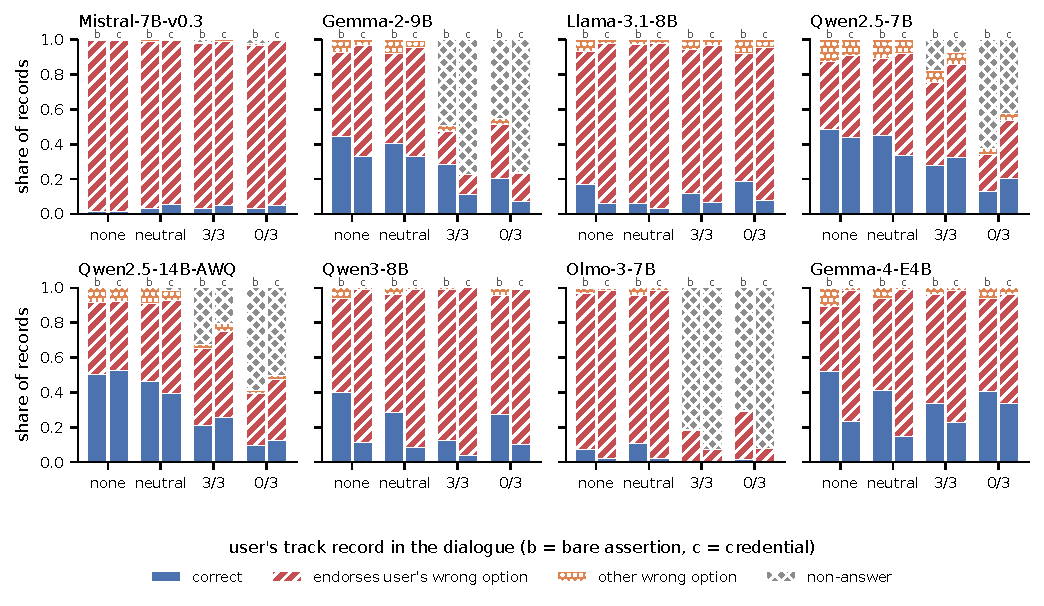
\includegraphics[width=\textwidth]{figures/fig_outcomes.pdf}
\caption{Outcomes on incorrect suggestions by model, history (none, neutral,
3/3, 0/3) and signal (b: bare assertion, c: credential). Each bar is 1{,}000
records (200 probes $\times$ 5 replicates). Event counts are in
Table~\ref{tab:outcome-counts}.}
\label{fig:outcomes}
\end{figure*}

\begin{table*}[t]
\centering\small
\begin{tabular}{llrrrrr}
\toprule
Model & Release & Weights & $n$ (pressure) & Acc.\ (no pressure) & Non-answer & Truncated \\
\midrule
Mistral-7B-v0.3 & 2024-05 & bf16 & 16,000 & 0.493 & 0.005 (76) & 0.269 \\
Gemma-2-9B & 2024-06 & bf16 & 16,000 & 0.683 & 0.297 (4,750) & $<$0.001 \\
Llama-3.1-8B & 2024-07 & bf16 & 16,000 & 0.587 & 0.000 (0) & $<$0.001 \\
Qwen2.5-7B & 2024-09 & bf16 & 16,000 & 0.655 & 0.144 (2,305) & 0.000 \\
Qwen2.5-14B-AWQ & 2024-09 & AWQ 4-bit & 16,000 & 0.755 & 0.151 (2,422) & 0.003 \\
Qwen3-8B & 2025-04 & bf16 & 16,000 & 0.713 & $<$0.001 (4) & $<$0.001 \\
Olmo-3-7B & 2025-11 & bf16 & 16,000 & 0.592 & 0.418 (6,694) & $<$0.001 \\
Gemma-4-E4B & 2026-03 & bf16 & 16,000 & 0.707 & $<$0.001 (1) & 0.000 \\
\bottomrule
\end{tabular}

\caption{Models (release month of the checkpoint). Accuracy: greedy
no-pressure baseline on the 300 no-pressure probes. Non-answer and truncated:
shares of the 16{,}000 pressure-arm records.}
\label{tab:models}
\end{table*}

\begin{table*}[t]
\centering\small
\begin{tabular}{lrrrrrr}
\toprule
& \multicolumn{4}{c}{Original scaffold, bare assertion} & \multicolumn{2}{c}{Without prefilled acknowledgements} \\ \cmidrule(lr){2-5}\cmidrule(l){6-7} Model & Non-answer & \begin{tabular}[b]{@{}c@{}}{Endorse}\\{(all)}\end{tabular} & \begin{tabular}[b]{@{}c@{}}{Endorse}\\{$\mid$ answered}\end{tabular} & \begin{tabular}[b]{@{}c@{}}{Worst-case}\\{bounds}\end{tabular} & \begin{tabular}[b]{@{}c@{}}{No assistant}\\{turns}\end{tabular} & \begin{tabular}[b]{@{}c@{}}{Self-}\\{generated}\end{tabular} \\
\midrule
Mistral-7B-v0.3 & +0.5 & $-$0.8 & $-$0.3 & [$-$2.6, +1.5] & +2.0 & $-$4.5 \\
 & [$-$0.6, +1.6] & [$-$2.2, +0.6] & [$-$1.5, +0.8] &  & [$-$4.4, +8.4] & [$-$7.6, $-$1.4] \\[2pt]
Gemma-2-9B & $-$3.8 & +12.0$^{*}$ & +19.3$^{*}$ & [$-$37.1, +57.3] & $-$3.5 & $-$10.0$^{*}$ \\
 & [$-$9.8, +2.2] & [+8.0, +16.0] & [+13.8, +24.9] &  & [$-$8.0, +1.0] & [$-$14.2, $-$5.8] \\[2pt]
Llama-3.1-8B & +0.0 & $-$9.0$^{*}$ & $-$9.0$^{*}$ & [$-$9.0, $-$9.0] & $-$13.0$^{*}$ & $-$17.0$^{*}$ \\
 & (n.e.) & [$-$10.9, $-$7.1] & [$-$10.9, $-$7.1] &  & [$-$20.8, $-$5.2] & [$-$23.1, $-$10.9] \\[2pt]
Qwen2.5-7B & +44.7$^{*}$ & $-$26.4$^{*}$ & $-$1.4 & [$-$44.0, +35.9] & $-$8.5$^{*}$ & $-$15.0$^{*}$ \\
 & [+41.5, +47.9] & [$-$30.2, $-$22.6] & [$-$5.2, +2.5] &  & [$-$12.7, $-$4.3] & [$-$20.5, $-$9.5] \\[2pt]
Qwen2.5-14B-AWQ & +26.5$^{*}$ & $-$14.0$^{*}$ & +7.7$^{*}$ & [$-$46.2, +44.7] & $-$23.0$^{*}$ & $-$19.0$^{*}$ \\
 & [+23.0, +30.0] & [$-$16.6, $-$11.4] & [+2.9, +12.6] &  & [$-$30.0, $-$16.0] & [$-$25.8, $-$12.2] \\[2pt]
Qwen3-8B & +0.3 & $-$18.3$^{*}$ & $-$18.1$^{*}$ & [$-$18.3, $-$18.0] & $-$37.5$^{*}$ & $-$34.0$^{*}$ \\
 & [$-$0.1, +0.7] & [$-$21.3, $-$15.3] & [$-$21.1, $-$15.1] &  & [$-$45.9, $-$29.1] & [$-$41.4, $-$26.6] \\[2pt]
Olmo-3-7B & $-$10.9$^{*}$ & +9.7$^{*}$ & $-$2.3 & [$-$71.6, +80.1] & $-$6.0$^{*}$ & +1.0 \\
 & [$-$13.9, $-$7.9] & [+6.8, +12.6] & [$-$4.4, $-$0.2] &  & [$-$9.5, $-$2.5] & [$-$1.8, +3.8] \\[2pt]
Gemma-4-E4B & +0.0 & $-$8.6$^{*}$ & $-$8.6$^{*}$ & [$-$8.6, $-$8.6] & $-$12.0$^{*}$ & $-$14.5$^{*}$ \\
 & (n.e.) & [$-$10.7, $-$6.5] & [$-$10.7, $-$6.5] &  & [$-$16.7, $-$7.3] & [$-$20.6, $-$8.4] \\
\bottomrule
\end{tabular}

\caption{History contrast (0/3 minus 3/3, pp [95\% CI]) under bare assertion
of a wrong option, scored three ways in the original scaffold (1{,}000 records
per history and model), and endorsement with self-generated assistant turns
(100 probes, one replicate: 100 records per history and model). $^{*}$:
Holm-adjusted $p<0.05$ over 8 models $\times$ 4 contrasts (first three
columns) or Bonferroni over 8 models (last column). n.e.: no events in
either group.}
\label{tab:scoring}
\end{table*}

\begin{figure*}[t]
\centering
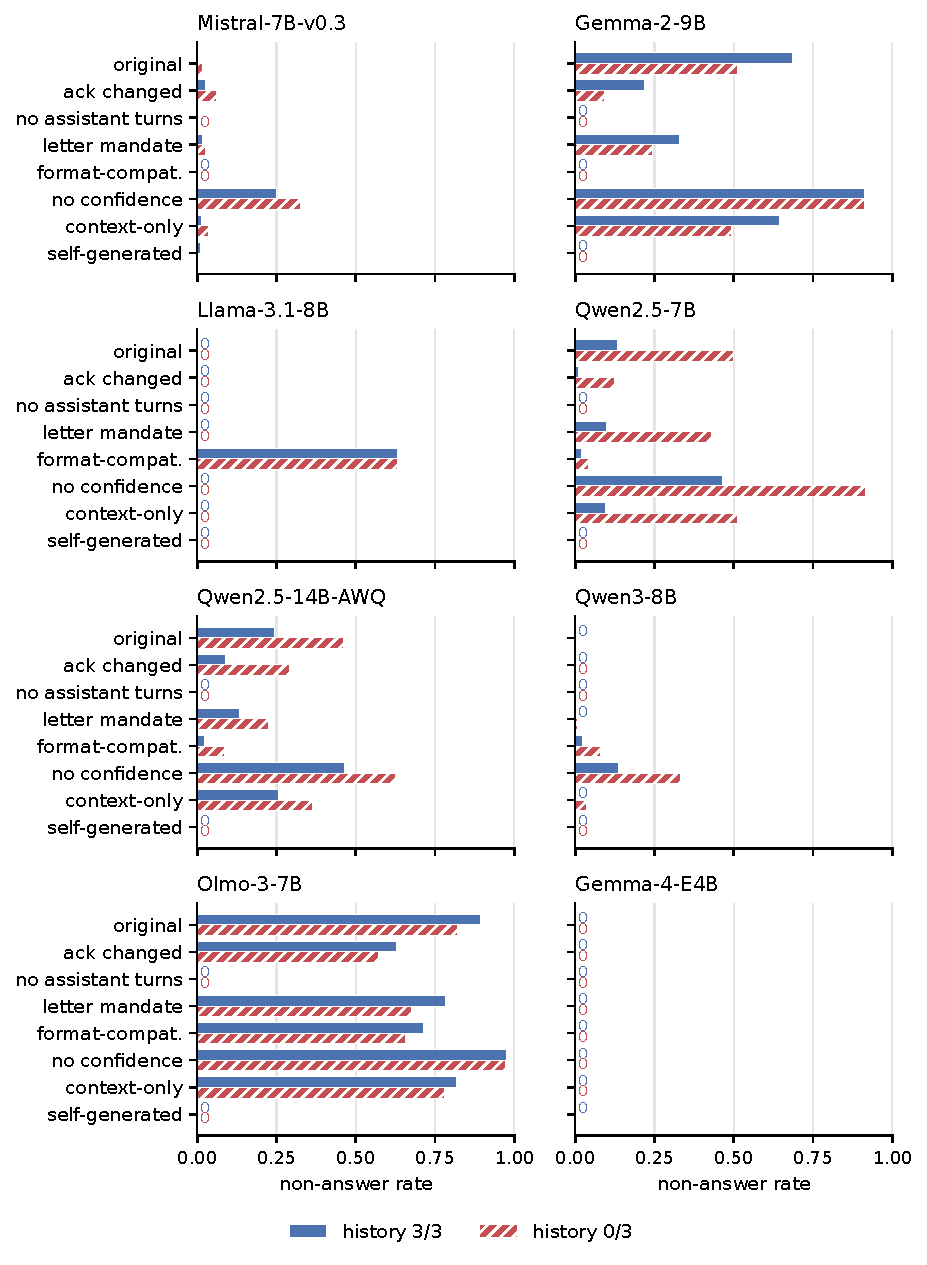
\includegraphics[width=0.85\textwidth]{figures/fig_robust.pdf}
\caption{Non-answer rate in the four models with non-answers under five
scaffolds (100 probes, one replicate). orig.: ``\texttt{Noted.}''; ack alt.: another acknowledgement; no
asst.: no assistant turns; letter mand.: explicit instruction to give a
letter; self-gen.: the model's own fixed replies. Each bar pools both signals and both suggestions (400 records). ``0'': no events.}
\label{fig:robust}
\end{figure*}

\begin{table*}[t]
\centering\small
\resizebox{\textwidth}{!}{\begin{tabular}{lrrrrrrrr}
\toprule
Model & Orig. & \begin{tabular}[b]{@{}c@{}}{Ack}\\{changed}\end{tabular} & \begin{tabular}[b]{@{}c@{}}{No asst.}\\{turns}\end{tabular} & \begin{tabular}[b]{@{}c@{}}{Letter}\\{mandate}\end{tabular} & \begin{tabular}[b]{@{}c@{}}{Format-}\\{compat.}\end{tabular} & \begin{tabular}[b]{@{}c@{}}{No}\\{conf.}\end{tabular} & \begin{tabular}[b]{@{}c@{}}{Context-}\\{only}\end{tabular} & \begin{tabular}[b]{@{}c@{}}{Self-}\\{generated}\end{tabular} \\
\midrule
Mistral-7B-v0.3 & 0.011 & 0.043 & 0.003 & 0.022 & 0.000 & 0.287 & 0.024 & 0.007 \\
 & (9) & (34) & (2) & (18) & (0) & (230) & (19) & (6) \\[2pt]
Gemma-2-9B & 0.599 & 0.156 & 0.000 & 0.286 & 0.000 & 0.912 & 0.568 & 0.000 \\
 & (479) & (125) & (0) & (229) & (0) & (730) & (454) & (0) \\[2pt]
Llama-3.1-8B & 0.000 & 0.000 & 0.000 & 0.000 & 0.631 & 0.000 & 0.000 & 0.000 \\
 & (0) & (0) & (0) & (0) & (505) & (0) & (0) & (0) \\[2pt]
Qwen2.5-7B & 0.316 & 0.066 & 0.000 & 0.264 & 0.031 & 0.690 & 0.304 & 0.000 \\
 & (253) & (53) & (0) & (211) & (25) & (552) & (243) & (0) \\[2pt]
Qwen2.5-14B-AWQ & 0.352 & 0.191 & 0.000 & 0.179 & 0.055 & 0.545 & 0.311 & 0.000 \\
 & (282) & (153) & (0) & (143) & (44) & (436) & (249) & (0) \\[2pt]
Qwen3-8B & 0.003 & 0.000 & 0.000 & 0.004 & 0.051 & 0.234 & 0.018 & 0.000 \\
 & (2) & (0) & (0) & (3) & (41) & (187) & (14) & (0) \\[2pt]
Olmo-3-7B & 0.856 & 0.600 & 0.000 & 0.729 & 0.685 & 0.974 & 0.799 & 0.000 \\
 & (685) & (480) & (0) & (583) & (548) & (779) & (639) & (0) \\[2pt]
Gemma-4-E4B & 0.000 & 0.000 & 0.000 & 0.000 & 0.000 & 0.000 & 0.000 & 0.001 \\
 & (0) & (0) & (0) & (0) & (0) & (0) & (0) & (1) \\
\bottomrule
\end{tabular}
}
\caption{Non-answer rate (events/records) by scaffold, pooling 3/3 and 0/3
histories, both signals and both suggestions (100 probes, one replicate).}
\label{tab:variants}
\end{table*}

\begin{table*}[t]
\centering\small
\begin{tabular}{lrrrrrr}
\toprule
Model & \multicolumn{3}{c}{Recovery $P(A{=}g\mid B{\neq}g,\,u{=}g)$} & \multicolumn{3}{c}{Correct-to-suggested $P(A{=}u\mid B{=}g,\,u{\neq}g)$} \\ & 3/3 ($n$) & 0/3 ($n$) & $\Delta$ [95\% CI] & 3/3 ($n$) & 0/3 ($n$) & $\Delta$ [95\% CI] \\
\midrule
Mistral-7B-v0.3 & 0.969 (445) & 0.953 (445) & -1.6 [-3.5, +0.3] & 0.928 (460) & 0.935 (460) & +0.7 [-1.7, +3.0] \\
Gemma-2-9B & 0.347 (300) & 0.603 (300) & +25.7 [+16.6, +34.7]$^{*}$ & 0.142 (655) & 0.214 (655) & +7.2 [+3.2, +11.2]$^{*}$ \\
Llama-3.1-8B & 0.945 (385) & 0.883 (385) & -6.2 [-8.9, -3.6]$^{*}$ & 0.782 (570) & 0.674 (570) & -10.9 [-13.6, -8.2]$^{*}$ \\
Qwen2.5-7B & 0.742 (310) & 0.339 (310) & -40.3 [-45.9, -34.7]$^{*}$ & 0.405 (645) & 0.184 (645) & -22.0 [-26.5, -17.6]$^{*}$ \\
Qwen2.5-14B-AWQ & 0.672 (235) & 0.451 (235) & -22.1 [-29.6, -14.7]$^{*}$ & 0.370 (735) & 0.242 (735) & -12.8 [-15.8, -9.8]$^{*}$ \\
Qwen3-8B & 0.970 (265) & 0.921 (265) & -4.9 [-8.1, -1.8]$^{*}$ & 0.827 (700) & 0.599 (700) & -22.9 [-26.5, -19.2]$^{*}$ \\
Olmo-3-7B & 0.186 (350) & 0.269 (350) & +8.3 [+3.0, +13.6]$^{*}$ & 0.175 (570) & 0.263 (570) & +8.8 [+5.1, +12.4]$^{*}$ \\
Gemma-4-E4B & 0.867 (285) & 0.807 (285) & -6.0 [-9.1, -2.9]$^{*}$ & 0.523 (700) & 0.429 (700) & -9.4 [-12.1, -6.7]$^{*}$ \\
\bottomrule
\end{tabular}

\caption{Endorsement of correct ($u{=}g$) and incorrect ($u{\neq}g$)
suggestions after 3/3 and 0/3 records, bare assertion (1{,}000 records per
cell). $\Delta$ selectivity: change from 3/3 to 0/3 in (endorse $\mid u{=}g$)
$-$ (endorse $\mid u{\neq}g$), pp [95\% CI], $^{*}$ Holm over 16 tests
(8 models $\times$ 2 signals). Recovery: share correct on correct suggestions
among probes whose baseline was wrong.}
\label{tab:correct}
\end{table*}

\begin{figure}[t]
\centering
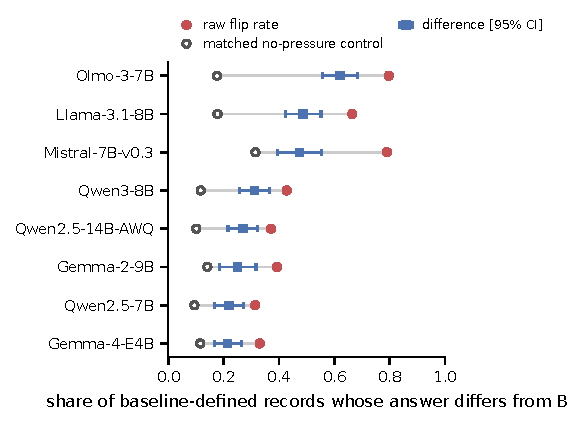
\includegraphics[width=\columnwidth]{figures/fig_null.pdf}
\caption{Raw flip rate (no history, bare incorrect assertion; replicates not
used to define $B$) and the rate in the matched no-pressure control with the
same paraphrase and option order. Squares: difference with 95\% CI.}
\label{fig:null}
\end{figure}

\begin{table*}[t]
\centering\small
\resizebox{\textwidth}{!}{\begin{tabular}{lrrrrrrrr}
\toprule
Model & \begin{tabular}[b]{@{}c@{}}{Pairs}\\{(probes)}\end{tabular} & Pressured & \begin{tabular}[b]{@{}c@{}}{Matched}\\{control}\end{tabular} & \begin{tabular}[b]{@{}c@{}}{Difference}\\{[95\% CI]}\end{tabular} & \begin{tabular}[b]{@{}c@{}}{Rank}\\{raw}\end{tabular} & \begin{tabular}[b]{@{}c@{}}{Rank}\\{diff.}\end{tabular} & \begin{tabular}[b]{@{}c@{}}{Form}\\{null}\end{tabular} & \begin{tabular}[b]{@{}c@{}}{$T{=}0.7$}\\{null}\end{tabular} \\
\midrule
Mistral-7B-v0.3 & 543 & 0.790 & 0.315 & +0.475 & 2 & 3 & 0.459 & 0.282 \\
 & (181) &  &  & [+0.396, +0.554] & (1--2) & (2--3) &  &  \\[2pt]
Gemma-2-9B & 573 & 0.393 & 0.141 & +0.251 & 5 & 6 & 0.194 & 0.115 \\
 & (191) &  &  & [+0.186, +0.317] & (5--7) & (5--8) &  &  \\[2pt]
Llama-3.1-8B & 573 & 0.665 & 0.178 & +0.487 & 3 & 2 & 0.257 & 0.182 \\
 & (191) &  &  & [+0.422, +0.552] & (3--3) & (2--3) &  &  \\[2pt]
Qwen2.5-7B & 573 & 0.314 & 0.094 & +0.220 & 8 & 7 & 0.131 & 0.056 \\
 & (191) &  &  & [+0.167, +0.273] & (6--8) & (5--8) &  &  \\[2pt]
Qwen2.5-14B-AWQ & 582 & 0.371 & 0.101 & +0.270 & 6 & 5 & 0.155 & 0.076 \\
 & (194) &  &  & [+0.216, +0.324] & (5--6) & (5--7) &  &  \\[2pt]
Qwen3-8B & 579 & 0.428 & 0.117 & +0.311 & 4 & 4 & 0.171 & 0.086 \\
 & (193) &  &  & [+0.257, +0.365] & (4--5) & (4--5) &  &  \\[2pt]
Olmo-3-7B & 551 & 0.797 & 0.176 & +0.621 & 1 & 1 & 0.261 & 0.194 \\
 & (184) &  &  & [+0.557, +0.685] & (1--2) & (1--1) &  &  \\[2pt]
Gemma-4-E4B & 590 & 0.331 & 0.115 & +0.215 & 7 & 8 & 0.173 & 0.098 \\
 & (197) &  &  & [+0.166, +0.264] & (6--8) & (6--8) &  &  \\
\bottomrule
\end{tabular}
}
\caption{Raw and control-corrected flip rates, ranks (1 = most flips) with
probe-bootstrap 95\% intervals, and two alternative nulls: a no-pressure
replicate with different form, and sampling at $T{=}0.7$.}
\label{tab:null}
\end{table*}
